\section{Language-level Leakage Characterization}\label{sec:leakagePL}
In this section, we characterize the leakage of MPC applications from the language perspective.

\subsection{A Language for MPC}
%For the sake of presentation,
We consider a simple language {\LANG} for implementing MPC applications.
The syntax of {\LANG} programs is defined as follows. %, which is an extension of the \emph{while} language: % with a declassify operator {\Pdeclassify}.
\begin{align*}
  p  ::=  & {\Pskip} \mid x = e  \mid \ p_1; p_2 \mid   {\Pif} \ x \ {\Pthen} \  p_1 \ {\Pelse} \ p_2 \mid {\Preturn} \ x \\
    & \mid    {\Pwhile} \ x \ \Pdo \ p  \mid {\Prepeat} \ n \ \Pdo \ p
\end{align*}
where $e$ is an expression defined as usual and $n$ is a positive integer.

%and a secure integer type {\Psint}.
Despite its simplicity, {\LANG} suffices to illustrate our approach %describe a wide range of MPC applications
and our tool supports a real-world language. % and fully illustrate our approach.
Note that we introduce two loop constructs.
The {\Pwhile} loop can only be used with the secret-independent conditions
while the {\Prepeat} loop (with a fixed number $n$ of iterations) can have secret-dependent conditions.
%and secret-independent conditional statements.
The restriction of the {\Pwhile} loop
is necessary, as %argued by  Zahur and Evans
the adversary knows when to terminate the loop, so
secret information may be leaked if a secret-dependent condition is used~\cite{ZahurE15}.

The operational semantics of the {\LANG} program is defined in a standard way %using transitions between configurations
(cf.\  Appendix~\ref{sec:semantics}). %, as shown in Figure~\ref{fig:semantics}.
In particular, ${\Prepeat}$ $n$ $\Pdo$ $p$ means repeating the loop body $p$ for a fixed number $n$ times.
A \emph{configuration} is a tuple $\MPCAngle{p, \sigma}$, where $p$ denotes a statement and $\sigma:\Var\rightarrow\Dom$ denotes a state that maps variables to values.
The evaluation of an expression $e$ under a state $\sigma$ is denoted by $\sigma(e)$.
%
A transition from  $\MPCAngle{p, \sigma}$ to $\MPCAngle{p', \sigma'}$
is denoted by $\MPCAngle{p, \sigma}\rightarrow \MPCAngle{p', \sigma'}$ and $\rightarrow^*$ denotes the transitive closure of $\rightarrow$.
%
An \emph{execution} starting from the configuration $\MPCAngle{p, \sigma}$ is a sequence of configurations. We write $\MPCAngle{p, \sigma}\Downarrow \sigma'$
if $\MPCAngle{p, \sigma}\rightarrow^* \MPCAngle{{\Pskip}, \sigma'}$.
We assume that each execution ends in a {\Preturn} statement, i.e.,
all the {\Pwhile}\ loops always terminate.
We denote by $\MPCAngle{p, \sigma}\Downarrow \sigma':v$
the execution returning value $v$.


%%%%%%%%%%%%%%%%%%%%%%%%%%%%%%%%%%%%%%%%%%%%%%%%%%%%%%%%%%%%%%%%%%%%%%%%%%%%%%%%%%%%%

\subsection{Leakage Characterization in Ideal/Real-World}
An MPC application $f(\vec{x})$ is implemented as a {\LANG} program $p$.
An execution of the program $p$ evaluates the computation $f(\vec{x})$
as if a TTP directly executed the program $p$ on the private inputs.
In this setting, the adversary cannot observe any intermediate states of the execution %$\MPCAngle{p, \sigma}\Downarrow \sigma':v$,
other than the final result. % $v$.
%, where the initial state $\sigma$ maps the variables $\vec{x}$ to their private inputs.

Let $\Var^{\tt in}=\{x_1,\cdots,x_n\}\subseteq\Var$ be the set of private input variables.
We denote by $\InitState_0$ %: \Var^{\tt in}\rightarrow \Rng^n$
the set of the initial states.
Given a tuple of values $\vec{v}_k\in\Dom^k$  % for the private input variables $x_1,\cdots, x_k$,
and a result $v\in \Rng$, let $\leak_{\tt iw}^p(v,\vec{v}_k)$ % $\Sigma^p_{v,v_1,\cdots,v_k}$
denote the set of states $\sigma\in \InitState_0$ such that
$\MPCAngle{p, \sigma}\Downarrow \sigma':v$ for some state $\sigma'$ and $\sigma(x_i)=v_i$ for $1\leq i\leq k$.
Intuitively, when the adversary controls the parties $\Party{1},\cdots, \Party{k}$,
she learns the set of states $\leak_{\tt iw}^p(v,\vec{v}_k)$
from the result $v$ and the adversary-chosen private inputs $\vec{v}_k\in\Dom^k$.
%
%\tl{not quite understand this} For the adversary-chosen values $(v_1,\cdots, v_k)\in\Dom^k$ for the private inputs $x_1,\cdots, x_k$,
%the adversary cannot distinguish the initial states $\sigma\in\leak_{\tt iw}^p(v,v_1,\cdots,v_k)$ from the result $v$ in the ideal-world. %Therefore, $\leak_{\tt iw}^{v,v_1,\cdots,v_k}$ is the set of indistinguishable initial states to the adversary
%from the execution $\MPCAngle{p, \sigma}\Downarrow \sigma':v$  for any $\sigma\in \leak_{\tt iw}^{v,v_1,\cdots,v_k}$.
%We denote $\leak(\MPCAngle{p, \{x_1\mapsto v_1,\cdots,x_n\mapsto v_n\}}\Downarrow \sigma':v)$ the set of indistinguishable states $\Sigma^p_v(v_1,\cdots,v_k)$.
% and $\Sigma^f_v\subseteq \Sigma^f$ for a given value $v\in \Rng$ denote the set of initial states $\sigma$
%such that $\MPCAngle{p, \sigma}\Downarrow \sigma':v$ for some state $\sigma'$.
%For a given tuple of values $(v_1,\cdots,v_k)$ for the private inputs $(x_1,\cdots,x_k)$, let $\Sigma^f_v(v_1,\cdots,v_k)$ be the set
%of initial states $\sigma$ such that $\sigma\in\Sigma^f_v$
%and $\sigma(x_i)=v_i$ for all $1\leq i\leq k$.
We can reformulate the leakage of an MPC application $f(\vec{x})$ in the ideal-world (cf.\ Definition~\ref{def:leakageinIdeal})
as follows:


\begin{proposition}
Given an MPC application $f(\vec{x}_n)$  implemented by a program $p$,
$\vec{v}_n'\in\leak_{\tt iw}^f(v,\vec{v}_k)$
iff there exists a state $\sigma\in \leak_{\tt iw}^p(v,\vec{v}_k)$
such that $\sigma(x_i)=v_i'$ for $1\leq i\leq n$.
%
%the \emph{leakage} to the adversary of an execution $\MPCAngle{p, \sigma}\Downarrow \sigma':v$ from an initial state
%$\sigma\in \Sigma^f_v(v_1,\cdots,v_k)$ is the set of indistinguishable states $\Sigma^f_v(v_1,\cdots,v_k)$, where the values $(v_1,\cdots, v_k)\in\Dom^k$ of the private inputs $x_1,\cdots, x_k$ are chosen by the adversary.
\end{proposition}



%
%\begin{figure}[ht]
%    \centering
%  \begin{align*}
%%&  &  T::= & {\Pint} \mid {\Psint} \\
%&  &  p::= & {\Pskip} \mid x = e  \mid \ p_1; p_2 % \\ %\mid T\ x = {\Pdeclassify}(y)  \\ \mid  x = {\Pdeclassify}(e)
% \mid   {\Pif} \ x \ {\Pthen} \  p_1 \ {\Pelse} \ p_2 \mid {\Pwhile} \ x \ \Pdo \ p \mid {\Preturn} \ x
%    \end{align*}
%%    \vspace*{-4mm}
%    \caption{Syntax of {\LANG}}
%    \label{fig:syntax}
%\end{figure}

%
%\begin{figure}[ht]
%    \centering\footnotesize
%    \begin{tabular}{cc}
%%%%%%%%%%%%%%%%%%%%%%%%%%%%%%%%%%%%%%%%%%%
%    $\begin{array}{c}
%        \MPCState{e}{\sigma}=v \\
%        \hline
%        \MPCAngle{x=e, \sigma} \rightarrow_{\obv{\epsilon}} \MPCAngle{{\Pskip}, \sigma[x\mapsto v]}
%    \end{array}$ &
%%%%%%%%%%%%%%%%%%%%%%%%%%%%%%%%%%%%%%%%%%%
%   %    $\begin{array}{c}
%%        \MPCState{e}{\sigma}=v \\
%%        \hline
%%        \MPCAngle{T \ x = e, \sigma} \rightarrow_{\obv{\epsilon}}  \MPCAngle{{\Pskip}, \sigma[x\mapsto v]}
%%    \end{array}$ \\ \\
%%%%%%%%%%%%%%%%%%%%%%%%%%%%%%%%%%%%%%%%%%%
%       $\begin{array}{c}
%        \MPCState{y}{\sigma}=v \\
%        \hline
%        \MPCAngle{x = {\Pdeclassify}(y)} \rightarrow_{\obv{v}}  \MPCAngle{{\Pskip}, \sigma}
%    \end{array}$    \\ \\
%%%%%%%%%%%%%%%%%%%%%%%%%%%%%%%%%%%%%%%%%%%
%   $\begin{array}{c}
%        \MPCAngle{p_{1}, \sigma_{1}}             \rightarrow_{\obv{o_1}}      \MPCAngle{ {\Pskip}, \sigma_{2} } \quad
%        \MPCAngle{p_{2}, \sigma_{2}}    \rightarrow_{\obv{o_2}}   \MPCAngle{ p_{2}' , \sigma_{3} } \\
%        \hline
%        \MPCAngle{p_{1};p_{2}, \sigma_{1}}       \rightarrow_{\obv{o_1\cdot o_2}}     \MPCAngle{p_{2}', \sigma_{3}}
%    \end{array}$ &
%%%%%%%%%%%%%%%%%%%%%%%%%%%%%%%%%%%%%%%%%%%
%    $\begin{array}{c}
%        \MPCAngle{p_1,\sigma_{1}}    \rightarrow_{\obv{o}}    \MPCAngle{ p_1', \sigma_{2}}    \quad     p_{1}' \neq {\Pskip} \\
%        \hline
%        \MPCAngle{p_{1} ; p_{2}, \sigma_{1}} \rightarrow_{\obv{o}}  \MPCAngle{p_1^{\prime};p_2, \sigma_{2}}
%    \end{array}$  \\ \\
%%%%%%%%%%%%%%%%%%%%%%%%%%%%%%%%%%%%%%%%%%%
% $\begin{array}{c}
%        p= \MPCState{e}{\sigma} \ ? \ p_1 : \ p_2 \\
%        \hline
%        \MPCAngle{{\Pif} \ e \ {\Pthen} \  p_1 \ {\Pelse} \ p_2, \sigma}   \rightarrow_{\obv{\MPCState{e}{\sigma}}}   \MPCAngle{p,\sigma}
%    \end{array} $ &
%%%%%%%%%%%%%%%%%%%%%%%%%%%%%%%%%%%%%%%%%%%
%   $ \begin{array}{c}
%        p'=\MPCState{e}{\sigma} \ ? \ p;\text{while } e \text{ do } p \ : \ {\Pskip} \\
%        \hline
%        \MPCAngle{{\Pwhile} \ e \ \Pdo \ p, \sigma}\rightarrow_{\obv{\MPCState{e}{\sigma}}}  \MPCAngle{p',\sigma}
%    \end{array}$  \\ \\
%            $\begin{array}{c}
%        \MPCState{x}{\sigma}=v \\
%        \hline
%        \MPCAngle{{\Preturn} \ x)} \rightarrow_{\obv{v}} \MPCAngle{{\Pskip}, \sigma}
%    \end{array}$    &
%%%%%%%%%%%%%%%%%%%%%%%%%%%%%%%%%%%%%%%%%%%    \\
%    \end{tabular}
%    \caption{Semantics of {\LANG}}
%    \label{fig:semantics}
%    % instrumented semantics
%\end{figure}
%
%We first define the sequential semantics of {\LANG}  which is used to evaluate a secure multi-party computation $f$
%as if a trust-third-party (TTP) directly computes $f$ over the input data.
%The ideal-world semantics is defined using transitions between configurations, as shown in Figure~\ref{fig:semantics}.
%A configuration is a tuple $\MPCAngle{p, \sigma}$, where $p$ denotes a statement and $\sigma$ denotes a state that maps from variables to values.
%The evaluation of an expression $e$ under a state $\sigma$ is denoted by $\MPCState{e}{\sigma}$.
%A transition from a configuration $\MPCAngle{p, \sigma}$ to a configuration $\MPCAngle{p', \sigma'}$
%is denoted by $\MPCAngle{p, \sigma}\rightarrow_{\obv{o}} \MPCAngle{p', \sigma'}$, where $\obv{o}$ denotes the observation of the transition.
%We denote by $\rightarrow^*$ the transitive closure of $\rightarrow$, where observation is concatenated into an
%observation traces. An execution starting from a configuration $\MPCAngle{p, \sigma}$ ends in the state
%$\sigma'$ with observation trace $\obv{o}$ is written as $\MPCAngle{p, \sigma}\Downarrow_{\obv{o}} \sigma'$,
%if $\MPCAngle{p, \sigma}\rightarrow_{\obv{o}} \MPCAngle{{\Pskip}, \sigma'}$.


%\subsection{Leakage Characterization in Real-World}
We use security policies to characterize the leakage of MPC applications in the real-world.
%instead of modeling concrete MPC protocols,

%to characterize leakage of MPC applications in the real-world.


%\smallskip
\noindent{\bf Security level.}
%To define security policies,
We consider a lattice of security levels $\seclev=\{\Sec,\Pub\}$
with $\Pub \sqsubseteq\Pub$, $\Pub \sqsubseteq\Sec$, $\Sec \sqsubseteq\Sec$
and $\Sec \not\sqsubseteq\Pub$.
We denote by $\ell_1\sqcup\ell_2$ the least upper bound of
two security levels $\ell_1,\ell_2\in\seclev$, namely,
$\ell\sqcup \Sec = \Sec\sqcup \ell=\Sec$ for $\ell\in\seclev$
and $\Pub\sqcup \Pub=\Pub$.


%\smallskip
%\noindent{\bf Security policy.}
%Fix an MPC application $f(\vec{x}_n)$ whose
%functionality is implemented by a program $p$.


\begin{definition}
A \emph{security policy} $\varrho:\Var\rightarrow \seclev$ for the MPC application $f(\vec{x})$ is a function that associates each variable $x\in \Var$ with a security level $\ell\in \seclev$.
\end{definition}

Given a security policy $\varrho$ and a security level $\ell\in \seclev$,
let $\Var^\ell:=\{x\mid \varrho(x)=\ell\}\subseteq \Var$, i.e., the set of
variables with the security level $\ell$ under $\varrho$.
We lift the order $\sqsubseteq$ to security policies, namely, $\varrho\sqsubseteq\varrho'$  if $\varrho(x)\sqsubseteq\varrho'(x)$ for each $x\in \Var$.
%
When executing the program $p$ with a security policy $\varrho$ using an MPC protocol $\pi$, we assume that
the adversary can observe the values of the public variables $x\in \Var^{\Pub}$,
but not that of the secret variables $x\in \Var^{\Sec}$. This is a practical assumption and can be  well-supported by the existing approach.
For instance, Obliv-C~\cite{ZahurE15} allows developers to define an MPC application in an extension of C language, when compiled and linked, the result will be a concrete garbled circuit protocol $\pi_p$ whose computation does not reveal the values of any oblivious-qualified variables.
Thus, all the secret variables specified by the security policy $\varrho$ can be declared as oblivious-qualified variables in Obliv-C,
while all the public variables specified by the security policy $\varrho$ are declared without oblivious-qualification.
Similarly,
MPyC~\cite{MPyC20} is a Python package for implementing MPC applications that allows programmers to define instances of secret-typed variable classes using Python's class mechanism.
When executing MPC applications, instances of secret-typed class variables are protected via Shamir's secret sharing protocol~\cite{Shamir79}.
Thus, all the secret variables specified by the security policy $\varrho$ can be declared as instances of secret-typed variable classes in MPyC,
while all the public variables specified by the security policy $\varrho$ are declared as instances of Python's standard classes.
%We assume that the underlying MPC protocol $\pi$ is secure, namely,
%for every IFP $\varrho:\Var\rightarrow \seclev$,
%the adversary cannot observe the values of secret variables $x\in \Var^{\Sec}$,
%but can observe the values of public variables $x\in \Var^{\Pub}$
%when executing the program $p$ under the protocol $\pi$.
%%
%We argue that this assumption is feasible. \tl{what is the logic link here?}
%For instance, Obliv-C allows developers to define a SPMC application in an extension of C language, when compiled and linked,
%the result will be a concrete garbled circuit protocol $\pi_p$ whose computation does not reveal
%the values of any oblivious-qualified variables~\cite{ZahurE15}.
%Thus, all the variables associated with $\Sec$ in the IFP $\varrho$ can be declared as oblivious-qualified variables in Obliv-C,
%while all the variables associated with $\Pub$ in the IFP $\varrho$ are declared without oblivious-qualification.
%\fu{Add more examples.}


\smallskip
\noindent{\bf Leakage under a security policy.}
Fix a security policy $\varrho$ for the program $p$. Remark that the values of the secret variables will not be known even at runtime for each party, as they are encrypted.
This means that, unlike the secret-independent conditions, the secret-dependent conditions cannot be executed normally, and thus should be removed using, e.g., multiplexers, before transforming into circuits.
%In contrast, the truth value of each secret-independent conditions will be known at runtime for each party
%so that the circuit of branches are to be generated at runtime. %instead of the whole conditional statement.
%Therefore, to define the leakage of the program $p$ under the policy $\varrho$, we first have
%to remove secret-dependent conditions.
%Furthermore, while loops should also be unfolded.
%We denote by ${\sf unfold}(p)$ the program $p$ after loop unfolding.
%Note that in this work we only consider bounded loops, i.e., each loop is bounded
%by a public constant otherwise the loop condition will leak.
%These statements are removed by
%Formally,
We define the transformation $\Enc_\varrho(\cdot,\cdot)$, where $c$ is the selector of a multiplexer.
%which is recursively defined as follows:
{\small\begin{align*}
   &  \Enc_\varrho(c,p_1; p_2)\triangleq\Enc_\varrho(c,p_1);\Enc_\varrho(c,p_2) \qquad\qquad \quad\quad~~ \Enc_\varrho(c,{\Preturn} \ x)\triangleq {\Preturn} \ x \\
%%%%%%%%%%%%%%%%%%%%%%%%%%%%
%   & \Enc_\varrho(c,x = e)\triangleq
%            \left\{
%              \begin{array}{ll}
%                 x=e, & \hbox{if $c=1$;} \\
%                x= x+ c\times (e-x), & \hbox{otherwise.}
%              \end{array}
%            \right.\\
   & \Enc_\varrho(c,x = e)\triangleq x= x+ c\times (e-x)  \qquad \qquad \qquad\Enc_\varrho(c,\Pskip)\triangleq \Pskip  \\
%%%%%%%%%%%%%%%%%%%%%%%%%%%%
  & \Enc_\varrho(c,{\Pif} \ x \ {\Pthen} \  p_1 \ {\Pelse} \ p_2 )\triangleq
\left\{
  \begin{array}{ll}
    {\Pif} \ x \ {\Pthen} \  \Enc_\varrho(1,p_1) \ {\Pelse} \ \Enc_\varrho(1,p_2), & \hbox{if $c=1\wedge\varrho(x)=\Pub$;} \\
   \Enc_\varrho(c\& x, p_1);\Enc_\varrho(c\& \neg x, p_2), & \hbox{otherwise.}
  \end{array}
\right. \\
%%%%%%%%%%%%%%%%%%%%
  & \Enc_\varrho(c,{\Pwhile} \ x \ \Pdo\ p)\triangleq
            \left\{
              \begin{array}{ll}
               {\Pwhile} \ x \ \Pdo\ \Enc_\varrho(1,p), & \hbox{if $c=1\wedge\varrho(x)=\Pub$;} \\
               \textcolor{red}{\tt Error}, & \hbox{otherwise.}
              \end{array}
            \right. \\
&   \Enc_\varrho(c,{\Prepeat} \ n \ \Pdo\ p)\triangleq {\Prepeat} \ n \ \Pdo\ \Enc_\varrho(c,p)
\end{align*}}
%\tl{it seems that $\Enc_\varrho(c,x = e)$ does not need case distinction?}
Intuitively, %$\Enc(c,{\Pif} \ x \ {\Pthen} \  p_1 \ {\Pelse} \ p_2 )$ removes the
%secret-dependent conditional statement while preserves the conditional semantics.
%Our transformation $\Enc_\varrho(\cdot,\cdot)$ takes into account both control-flow and data-flow of information from private inputs.
$\Enc(c,x = e)$ simulates a multiplexer with two different values
depending on whether the assignment $x = e$ is in the scope of some secret-dependent conditions.
At runtime, the value $e$ is assigned to $x$ if $c$ is $1$, otherwise $x$ does not change.
$\Enc_\varrho(c,{\Pwhile} \ x \ \Pdo\ p)$ enforces that the {\Pwhile}\ loop is used in secret-independent conditions
and $x$ is public in the security policy $\varrho$ otherwise throws an error.
The other cases are trivial.
We denote by $\widehat{p}_\varrho$ the program $\Enc_\varrho(1,p)$ on which
we will define the leakage of $p$ in the real-world.
%To make intermediate computation results explicit, we assume that $p_\varrho$



For every state $\sigma: \Var\rightarrow \Rng$,
let $\sigma^{\Pub}:\Var^{\Pub}\rightarrow\Rng$ denote the
state that is the projection of the state $\sigma$ onto the public variables $\Var^{\Pub}$.
For each execution $\MPCAngle{\widehat{p}_\varrho, \sigma_1}\Downarrow \sigma_2$,  we denote
by $\MPCAngle{\widehat{p}_\varrho,\sigma_1}\Downarrow_\varrho^{\Pub} \sigma_2$ the sequence
of configurations where each state $\sigma$ %in the execution $\MPCAngle{\widehat{p}_\varrho, \sigma_1}\Downarrow \sigma_2$
is replaced by the state $\sigma^{\Pub}$.

Recall that the adversary can observe the values of public variables $x\in \Var^{\Pub}$
when executing the program $\widehat{p}_\varrho$. %  under the protocol $\pi$.
Thus, from an execution $\MPCAngle{\widehat{p}_\varrho,\sigma_1}\Downarrow\sigma_2:v$,
she can observe the sequence $\MPCAngle{\widehat{p}_\varrho,\sigma_1}\Downarrow_\varrho^{\Pub} \sigma_2$ and the result $v$, written as $\MPCAngle{\widehat{p}_\varrho,\sigma_1}\Downarrow_\varrho^{\Pub} \sigma_2:v$.
%
%Suppose the adversary chooses the values $(v_1,\cdots, v_k)\in\Dom^k$ for the private inputs $x_1,\cdots, x_k$
%and $\sigma_1\in\Sigma^p_v(v_1,\cdots,v_k)$,
%
For every state $\sigma\in\leak_{\tt iw}^p(v,\vec{v}_k)$,
we denote by $\leak_{\tt rw}^{p,\varrho}(v,\sigma)$
the set of states $\sigma'\in\leak_{\tt iw}^p(v,\vec{v}_k)$ such that
$\MPCAngle{\widehat{p}_\varrho,\sigma'}\Downarrow_\varrho^{\Pub} \sigma_1':v$
and $\MPCAngle{\widehat{p}_\varrho,\sigma}\Downarrow_\varrho^{\Pub} \sigma_1:v$ are identical.
%Given the adversary-chosen values $(v_1,\cdots, v_k)\in\Dom^k$ for the private inputs $x_1,\cdots, x_k$,
%let $\Sigma^{p,\varrho}_{\sigma,v_1,\cdots, v_k}$ be the set of initial states
%$\sigma'\in \Sigma^{p,\varrho}_{\sigma}$ such that $\sigma'(x_i)=v_i$ for $1\leq i\leq k$.



%
%
%Thus, observing the values of the public variables $\Var_\varrho^{\tt pub}$ in the intermediate computations of
%an execution $\MPCAngle{p, \sigma}\Downarrow \sigma'$ from an initial state
%$\sigma\in \Sigma^f$ is the same as observing the values of the public variables in the final
%state $\sigma'$. For a given state $\sigma$ and IFP $\varrho$, we denote by $\sigma_{\downharpoonright_{\varrho}^{\tt pub}}$
%the projection of the state $\sigma$ onto the public variables $\Var_\varrho^{\tt pub}$ defined in the IFP $\varrho$.
%For any valuation of the public variables $\beta:\Var_\varrho^{\tt pub}\rightarrow\Rng$,
%let $\Sigma^f_\beta\subseteq \Sigma^f$ denote the set of initial states
%$\sigma$ such that $\MPCAngle{p, \sigma}\Downarrow \sigma'$ and $\sigma'_{\downharpoonright_{\varrho}^{\tt pub}}=\beta$.
%Thus, observing the values of public variables in $\beta$ only reveals
%the set $\Sigma^f_\beta$.


\begin{definition}
A security policy $\varrho$ is \emph{perfect} for a given MPC application $f(\vec{x}_n)$ implemented by the program $p$, denoted by $\varrho\models_p f(\vec{x}_n)$,
if $\Enc_\varrho(1,p)$ does not throw any errors, and for adversary-chosen private inputs $\vec{v}_k\in\Dom^k$, the result $v\in\Rng$,
and the state $\sigma\in\leak_{\tt iw}^p(v,\vec{v}_k)$,
we have  that \[\leak_{\tt iw}^p(v,\vec{v}_k)=\leak_{\tt rw}^{p,\varrho}(v,\sigma).\]
%
%and for every initial state $\sigma\in \Sigma^f$,
%the \emph{leakage} of an execution $\MPCAngle{p, \sigma}\Downarrow \sigma'$ under the protocol $\pi$
%is the set of initial states $\Sigma^f_\beta$, where $\beta=\sigma'_{\downharpoonright_{\varrho}^{\tt pub}}$.
\end{definition}
%
Intuitively, a perfect security policy $\varrho$ ensures that
for every state $\sigma\in\leak_{\tt iw}^p(v,\vec{v}_k)$,
from the observation $\MPCAngle{\widehat{p}_\varrho,\sigma}\Downarrow_\varrho^{\Pub} \sigma':v$,
%of the execution $\MPCAngle{\widehat{p}_\varrho,\sigma_1}\Downarrow\sigma_2:v$,
the adversary only learns the same set
$\leak_{\tt iw}^p(v,\vec{v}_k)$ of initial states as that in the ideal-world.

Our goal is to compute a perfect security policy $\varrho$ for every program $p$ that implements
the MPC $f(\vec{x})$. A naive way %to compute a perfect policy $\varrho$
is to assign the high security level
$\Sec$ to all the variables $\Var$, which  %which definitively guarantees $\varrho\models_p f(\vec{x})$.
%However, this policy $\varrho$
may however suffer from a lower performance,
as all the intermediate computations have to be performed on encrypted data
and conditional statements have to removed.
Ideally, a security policy $\varrho$ should not only be perfect but also annotate as few secret variables as possible.


\begin{comment}
\subsection{Secure multi-party computation}

A secure multi-party computation is given by a function $f(x_1,\cdots, x_n)$ whose
function body is a statement $p$ in {\LANG}.


The goal of Secure Multi-party computation (MPC) is to enable a group of $n$ participants who do not trust each other or any third party to jointly compute a function $f(x_1,\cdots,x_n)$
where the $i$-th participant owns the private input $x_i$.
MPC ensures the computation process reveals nothing but the result of $f$ to participants.

Yao firstly introduced the MPC problem in the early 1980s \cite{EvansKR18}.
In \cite{yao82}, Yao proposed Yao's garbled circuit protocol for solving the MPC problem.
Goldreich et al. \cite{GMW} proposed an additive secret sharing approach to solve MPC.
A decade ago, Damg{\aa}rd et al. \cite{SHE} proposed a new MPC approach based on %a somewhat
homomorphic cryptosystems.
The above three protocols and their ideas became the basis of research work in the field of MPC protocol design.
Garbled circuits, secret sharing, and homomorphic encryption have become the base protocols for today's MPC implementations.
Due to the unresolved performance issues of homomorphic encryption, real-world MPC implementations tend to choose either garbled circuit-based protocols or secret-sharing-based protocols.
In the experiment section, we consider experiments on the implementation of these two protocols.

\subsection{Adversary and security model}
\subsubsection{Adversary model}
We consider a passive adversary who %A passive adversary are curious but honest attackers, also known as semi-honest adversary. A passive adversary
will execute the protocol honestly, but may try to get as much information as possible from the messages received by the other participants.
This means that a passive adversary can only try to get secret information by observing their own view during the execution of the protocol. % and cannot take any other attack action.

The adversary in MPC is also a participant in the computation.
We consider multiple colluding adversaries as an adversary who corrupts multiple participants.

% Another class of adversaries is the active adversary, also called malicious adversary.
% The active adversary can make the corrupted participants deviate from the protocol rules to execute the protocol at will.
% A active adversary has the same ability to analyze the protocol execution process as a passive adversary,
% but a malicious adversary can take arbitrary attack actions during the protocol execution, such as controlling the network and interrupting the protocol execution.

\subsubsection{Security model}
MPC security is described in a real-ideal paradigm.
Real-ideal paradigm introduces a well-defined ideal world that covers all security requirements, and defines security by discussing the relationship between the real world and the ideal world.
The Figure \ref{fig:real-ideal} explains the difference between the real world and the ideal world.

\begin{figure}[h]
    \centering
    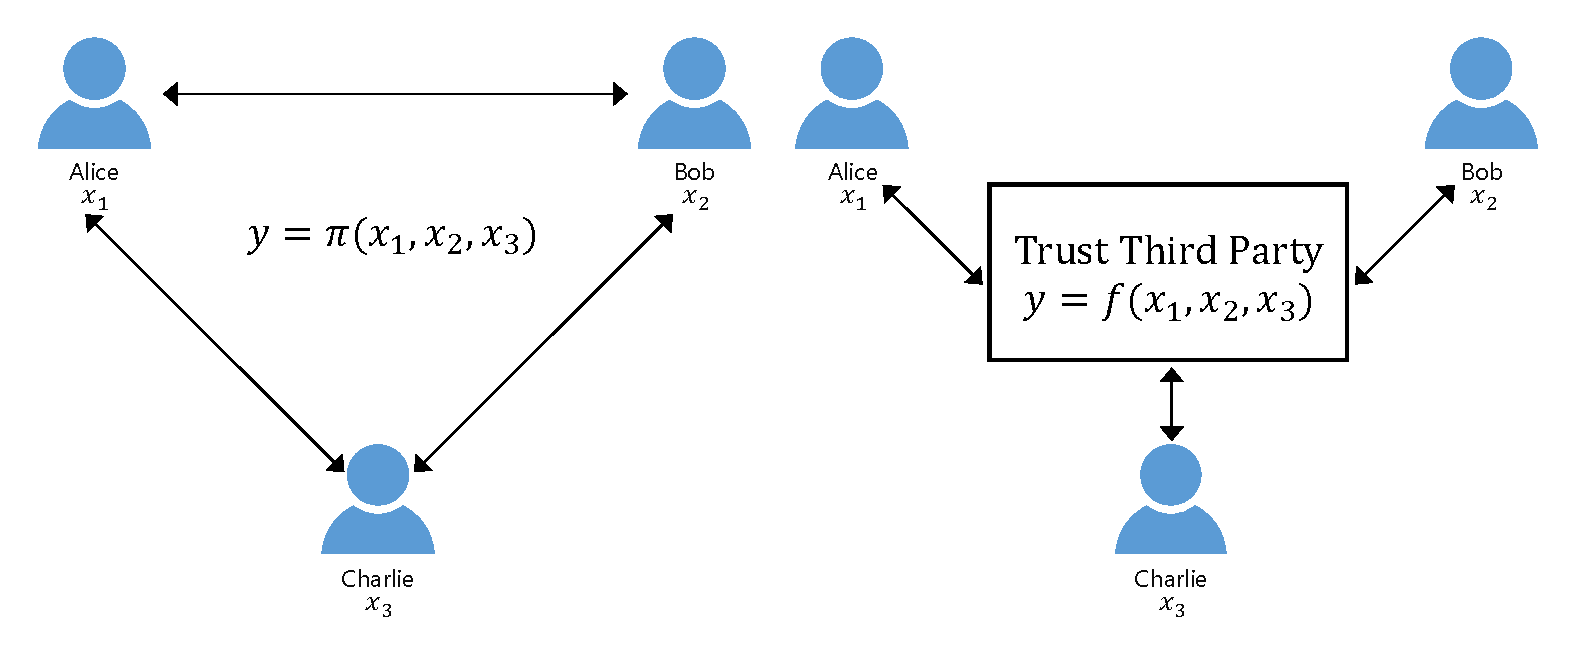
\includegraphics[scale=0.33]{img/real-ideal.pdf}
    \caption{Real-world vs. Ideal-world}
    \label{fig:real-ideal}
\end{figure}



In the real world, all participants communicate with each other through the protocol $\pi$.
Participant $P_i$ generates the message to be sent in the next communication round through the rules of the protocol $\pi$.
% based on the security parameters, random tape, private input $x_i$ and all messages received so far .
At the end of the protocol execution, participants will give output according to the rules of the protocol.

In the ideal world, each participant $P_i$ secretly sends its private input $x_i$ to a TTP %fully trusted third party $\mathcal{T}$.
The $\mathcal{T}$ securely compute $y=f(x_1,...,x_n)$ and returns the result to all participants.


The view of participant $P_i$ consists of its private input $x_i$, random tape, and all messages received during the protocol execution.
An adverasry's view consists of views of all corrupt parties.
The ideal world uses an simulator \textit{Sim} to simulate the participant $P_i$'s view.
The \textit{Sim} receives private input $x_i$ and the result, output the view of each $P_i$.
If the views of the adversary in the real world is indistinguishable from the views of adversary in the ideal world,
then the protocol $\pi$ is secure under the attack of a passive adversary.


The attack action of a passive adversary is to output its entire view.

Let $\pi$ be the MPC protocol evaluating the function $f$, $k$ be the security parameter, $\mathcal{C}$ be the set of corrupted participants, %of the adversary,
and $V_i$ (resp. $\textit{Sim}(x_i, y)$) be the view of the participant $P_i$ in the real (resp. ideal) world.
We define the probability distribution \tl{??} of the following two random variables:
\begin{itemize}
    \item $\text{Real}_{\pi}(k, \mathcal{C};x_1,\cdots,x_n):$ Participants execute protocol $\pi$  with the security parameter $k$ honestly over their private inputs $x_1,\cdots,x_n$. \\
    Outputs $\{V_i\mid  i\in \mathcal{C}\}$.
    \item $\text{Ideal}_{f,\textit{Sim}}(k, \mathcal{C};x_1,\cdots ,x_n):$ The trust party computes $y=f(x_1,\cdots,x_n)$.\\
    Outputs $\{\textit{Sim}(x_i,y)\mid i\in \mathcal{C}\}$.
\end{itemize}

\begin{definition}[Passive security]
    A protocol $\pi$ securely implements the function $f$ in the presence of a passive adversary if there exists a simulator \textit{Sim}
    such that, for all subsets of the corrupted participants set $\mathcal{C}$, the probability distributions
    \[\text{Real}_{\pi}(k, \mathcal{C};x_1,\cdots,x_n) \]
    and
    \[\text{Ideal}_{f,\textit{Sim}}(k, \mathcal{C};x_1,\cdots,x_n)\]
    are indistinguishable (in $k$) \tl{needs to be defined?} for all inputs $x_1,\cdots,x_n$.
\end{definition}


%%%%%%%%%%%%%%%%%%%%%%%%%%%%%%%%%%%%%%%%%%%%%%%%%%%%%%%%%%%%%%%%%%%%%%%%%%%%%%%%%%%%%%%%%%%%%%%%%%%%%%%%%%%%%



%\subsubsection{Privacy type system}
%Figure \ref{type} shows the type system of public and secret variables. $\mathbb{P}$ denotes public type and $\mathbb{S}$ denotes secret type.
%Oblivious RAM (ORAM) \cite{ORAM} is a memory abstraction that allows arbitrary memory access without leaking any information about which locations are accessed.
%MPC programs can access an array item by secret index using ORAM without leaking the index value.
%
%Our privacy type system statically assigns privacy type to variables.
%The privacy environment $\Gamma:V \rightarrow \mathcal{L}$ is a mapping from variable to privacy types where $V$ is the set of variables and $\mathcal{L}=\{\mathbb{P},\mathbb{S}\}$ with $\mathbb{P}\sqsubseteq \mathbb{S}$.
%We  summarize several rules of the privacy type system in Figure \ref{type}:
%\begin{enumerate}
%    \item Public variables can be assigned to secret variables, but not vice versa.
%    \item \textit{reveal} operator convert secret variables to public variables.
%    \item Secret variable can be as the index of ORAM array.
%    \item The control flow of while-statement and if-statement depends on public variables while Obliv if-statement use secret variables as control flow condition.
%\end{enumerate}
%To avoid the occurrence of side-channel, we assume that the statements in the oblivious control structure can read but not write to outer scope public variable.
%
%\begin{figure}[ht]
%    \centering
%    \label{type}
%    \[
%    \begin{array}{cc}
%        \text{Sequence} \\
%        \Gamma \vdash p_1 \quad \Gamma \vdash p_2 \\
%        \hline
%        {\Gamma \vdash p_1;p_2  }
%    \end{array}
%    \quad
%    \begin{array}{c}
%        \text{While} \\
%        \Gamma \vdash e : \mathbb{P} \quad \Gamma \vdash p \\
%        \hline
%        {\Gamma \vdash \text{while } e \text{ do } p }
%    \end{array}
%    \]
%    \[
%    \begin{array}{c}
%        \text{If} \\
%        \Gamma \vdash e : \mathbb{P} \quad \Gamma \vdash p_1 \quad \Gamma \vdash p_2 \\
%        \hline
%        {\Gamma \vdash \text{if } e \text{ then } p_1 \text{ else } p_2 }
%    \end{array}
%    \]
%    \[
%    \begin{array}{c}
%        \text{Obliv If} \\
%        \Gamma \vdash e : \mathbb{S} \quad \Gamma \vdash p_1 \quad \Gamma \vdash p_2 \\
%        \hline
%        {\Gamma \vdash \text{Obliv if } e \text{ then } p_1 \text{ else } p_2 }
%    \end{array}
%    \]
%    \[
%    \begin{array}{c}
%        \text{BinOp} \\
%        \Gamma \vdash e_1: \tau_1 \quad \Gamma \vdash e_2: \tau_2 \quad \tau_2 \sqsubseteq \tau_1\\
%        \hline
%        {\Gamma \vdash e_1 \text{ op } e_2: \tau_1  }
%    \end{array}
%    \]
%    \[
%    \begin{array}{c}
%        \text{\small{Neg}} \\
%        \Gamma \vdash e: \tau \\
%        \hline
%        {\Gamma \vdash \neg e: \tau  }
%    \end{array}
%    \quad
%    \begin{array}{c}
%        \text{\small{Reveal}} \\
%        \Gamma \vdash e: \mathbb{S} \\
%        \hline
%        {\Gamma \vdash \textit{reveal } e: \mathbb{P}  }
%    \end{array}
%    \]
%    \[
%    \begin{array}{c}
%            \text{Assign} \\
%            \Gamma \vdash lv : \tau_1 \quad \Gamma \vdash e : \tau_2 \quad \tau_2 \sqsubseteq \tau_1 \\
%            \hline
%            {\Gamma \vdash lv = e}
%        \end{array}
%    \]
%
%    \[
%    \begin{array}{c}
%        \text{Array Index} \\
%        \Gamma \vdash x: \text{Array}(\tau) \quad \Gamma \vdash i: \mathbb{P}\\
%        \hline
%        {\Gamma \vdash x[i] : \tau }
%    \end{array}
%    \quad
%    \begin{array}{cc}
%        \text{\small{Constant}} \\
%        \Gamma \vdash \diamond  \\
%        \hline
%        {\Gamma \vdash c: \mathbb{P}  }
%    \end{array}
%    \]
%    \[
%    \begin{array}{c}
%        \text{ORAM Index} \\
%        \Gamma \vdash x: \text{ORAM}(\tau) \quad \Gamma \vdash i: \mathbb{S}\\
%        \hline
%        {\Gamma \vdash x[i] : \tau }
%    \end{array}
%    \quad
%    \begin{array}{ll}
%        \text{\small{Skip}} \\
%        \Gamma \vdash \diamond  \\
%        \hline
%        {\Gamma \vdash \text{skip}  }
%    \end{array}
%    \]
%    \caption{Privacy type system}
%\end{figure}

\subsection{Information leakage of MPC}
%In the motivation example, we've been talking about private inputs and their information leakage.
%This subsection explains the private information and its leakage in detail .


\subsubsection{Intuition of private information and leakage}
%In the actual execution of an MPC protocol, the private information is the value of the private inputs.
%When analyzing information leakage, the private information is the distribution of the values of the private inputs.


Assume that before executing the MPC protocol, the adversary knows that the distribution of the participant $P_i$'s private input is $\Dom_{x_i}$.
After executing the MPC protocol, the adversary updates the distribution of the $P_i$'s private input to $D_{x_i}^\prime$ based on the information during the execution of the protocol.
If $D_{x_i}$ and $D_{x_i}^{\prime}$ are different, this MPC protocol leaks some private information of the private input.

Suppose the MPC protocol is secure, the evaluation of the MPC protocol still leak the result at least.
At the end of protocol evaluation, the result which is a secret variable is revealed to public the result to participants.
Information leakage cannot be completely avoided %such as the motivation example in Figure \ref{max3}.
In this work, we suppose the MPC protocol is secure and focus on the information leakage caused by publiced \tl{?} secret variables.



\subsubsection{Modeling Information leakage}
We model the information leakage from the knowledge of the adversary.
We formalize the knowledge of adversary learned from a MPC program as the partition of equivalence classes of private inputs.
For once protocol evaluation, the adversary learns the equivalence class contains the private inputs when observing the revealed secret variables.
\begin{definition}(Leakage trace)
    For an execution of MPC program $p$, $p$ reveals a secret variable $v$ who has semantic value $val$.
    The $expr_v$ is the symbolic expression of $v$ with respect to private inputs $x_1,...,x_n$.
    The information leakage of this \textit{reveal} operation is the constraint $\textit{Eq}(expr_v, val)$.
    The leakage trace of the execution of $p$ is the sequence of leakage of \textit{reveal} operations.
\end{definition}
\begin{definition}(Equivalence relation)
    The adversary cannot distinguish private input $x$ and $x'$,
    if the executions of MPC program $p(x)$ and $p(x')$ have the same leakage trace $l$,
    denotes $x\thicksim_{l} x'$
\end{definition}
\begin{definition}(Equivalence class)
    $X$ is the domain of $p$'s private inputs, an equivalence class $[\thicksim_{l}]$ is a subset of $X$ such that $[\thicksim_{l}]=\{x\in X| x \thicksim_{l} x', x'\in X, x' \not = x\}$
\end{definition}
\begin{definition}(Indistinguishable partition)
    The indistinguishable partition of $X$ is the set of all equivalence classes, $\{[\thicksim_l]|l \text{ is the leakage trace of a possible evaluation of } p\}$.
\end{definition}

The partition which is a set of equivalence classes can be equivalently represented by a set of constraints. Each constraint is corresponding to an equivalence class.
The constraints come from the path conditions of $p$'s control flow and the revealed secret variables.

Furthermore, the adversary can substitute its private input into the constraints to learn more accurate knowledge.
However, if the adversary learns a new indistinguishable partition which is the same as its owned indistinguishable partition from the execution of the program,
we ensure the adversary learns nothing from this execution.
\begin{definition}(Information leakage)
    For MPC program $p$ with private input $x\in X$,
    the information leakage of $p$ is the indistinguishable partition of $X$.
\end{definition}


%\subsection{Semantic}
%In our model, the semantic evaluates a MPC program like a trust third party with knowing all secret and public variables.
%The simulation of the trust third party simplifies our analysis and verification process.
%The semantics in Figure \ref{semantic} illustrates leakage trace of the program.
%
%We define semantics as the transitions between configurations.
%The execution of a program is a sequence of configuration transitions.
%A configuration is a pair  $\MPCAngle{p,\sigma }$ where $p$ is a program and $\sigma$ is a memory.
%Memory is a mapping, mapping variables $x$ or array element $x[i]$ to its semantic value $val$.
%The evaluation of expression $e$ under memory $\sigma$ is denoted as $\MPCState{e}{\sigma}$.
%$ \MPCAngle{p,\sigma}\rightarrow_{l} \MPCAngle{p^{\prime},\sigma^{\prime} }$  is a transition between two configurations,
%where $l$ is the leakage during the transition.
%Configuration $\MPCAngle{p,\sigma}$ terminates in memory $\sigma^\prime$ if $\MPCAngle{p,\sigma}\rightarrow^*\MPCAngle{\text{skip},\sigma^\prime}$.
%We write $\MPCAngle{p,\sigma}\Downarrow_{l} \sigma^\prime$ if configuration $\MPCAngle{p,\sigma}$ terminates in memory $\sigma^\prime$ with leakage $l$.
%
%
%\begin{figure}
%    \centering
%    $\begin{array}{c}
%        \MPCAngle{p_{1}, \sigma_{1}}             \rightarrow_{l}       \MPCAngle{ \text{skip}    , \sigma_{1}^{\prime} } \\
%        \MPCAngle{p_{2}, \sigma_{1}^{\prime}}    \rightarrow_{l^\prime} \MPCAngle{ p_{2}^{\prime} , \sigma_{2}^{\prime} } \\
%        \hline
%        \MPCAngle{p_{1};p_{2}, \sigma_{1}}       \rightarrow_{l \cdot l^{\prime}}    \MPCAngle{p_{2}^{\prime}, \sigma_{2}^{\prime}}
%    \end{array}$
%    \ \ \
%    $\begin{array}{c}
%        \MPCAngle{p_1,\sigma_{1}}    \rightarrow_{l}     \MPCAngle{ p_1^{\prime}, \sigma_{1}^{\prime} } \\
%        p_{1}^{\prime} \not = \text{skip} \\
%        \hline
%        \MPCAngle{p_{1} ; p_{2}, \sigma_{1}} \rightarrow_{l } \MPCAngle{p_1^{\prime};p_2, \sigma_{1}^{\prime}}
%    \end{array}$
%    \\
%    \[\begin{array}{c}
%        \MPCState{e}{\sigma}=val \\
%        \hline
%        \MPCAngle{lv := e, \sigma} \rightarrow \MPCAngle{\text{skip}, \sigma[lv\mapsto val]}
%    \end{array}\]
%    \\
%    \[\begin{array}{c}
%        p=\Big\{
%            \begin{array}{ll}
%            p_{1} & \text { if } \MPCState{e}{\sigma}=\text{true} \\
%            p_{2} & \text { if } \MPCState{e}{\sigma}=\text{false}
%            \end{array} \\
%        \hline
%        \MPCAngle{\text { if } e \text { then } p_{1} \text { else } p_{2}, \sigma}
%        \rightarrow
%        \MPCAngle{p,\sigma}
%    \end{array}\]
%    \\
%    \[\begin{array}{c}
%        p=\Big\{
%            \begin{array}{ll}
%            p_{1} & \text { if } \MPCState{e}{\sigma}=\text{true} \\
%            p_{2} & \text { if } \MPCState{e}{\sigma}=\text{false}
%            \end{array} \\
%        \hline
%        \MPCAngle{\text {obliv if } e \text { then } p_{1} \text { else } p_{2}, \sigma}
%        \rightarrow
%        \MPCAngle{p,\sigma}
%    \end{array}\]
%    \\
%    \[\begin{array}{c}
%        p^{\prime}=\Big\{
%            \begin{array}{ll}
%            p;\text{while } e \text{ do } p & \text { if } \MPCState{e}{\sigma}=\text{true} \\
%            \text{skip}                     & \text { if } \MPCState{e}{\sigma}=\text{false}
%            \end{array} \\
%        \hline
%        \MPCAngle{\text {while } e \text { do } p , \sigma}
%        \rightarrow
%        \MPCAngle{p^{\prime},\sigma}
%    \end{array}\]
%    \\
%    \[\begin{array}{c}
%        \MPCState{e}{\sigma}=val \\
%        \hline
%        \MPCAngle{lv := \text{reveal } e, \sigma}
%        \rightarrow_{\textit{Eq}(expr_{lv}, val)}
%        \MPCAngle{\text{skip}, \sigma[lv\mapsto val]}
%    \end{array}\]
%    \caption{Semantics}
%    \label{semantic}
%    % instrumented semantics
%\end{figure}
%
%We summarized a few rules from the semantics.
%\begin{enumerate}
%    \item Only \textit{reveal} statement contributes to leakage trace.\\
%    The \text{reveal} operator converts secret data to public data.
%    The semantic value of the secret data is revealed.
%    \item Obliv if-statement has no information leakage.\\
%    Obliv if-statement is an oblivious control structure.
%    The condition variable of an Obliv if-statement has a secret type.
%    Obliv if-statement executes then branch and else branch regardless of the value of the condition variable.
%    It uses multiplexers to selectively update variables based on the values of the conditional variable.
%    Participants cannot determine which branch Obliv if-statement executed.
%    \item if-statement and while-statement contribute nothing to leakage trace. \\
%    Even if the condition variable is a revealed secret variable, the leakage has already been traced at the \textit{reveal} statement.
%\end{enumerate}


\subsection{Information leakage lower bound}
MPC protects private inputs and is responsible for secure computation.
But MPC reveals the result of the secure computation program.
The functionality and the result of MPC program are public to participants makes the adversary have the ability to extract knowledge about others' private inputs.
MPC programs have a lower bound of information leakage, and this lower bound of information leakage cannot be avoided.

Suppose MPC program $p$ computes the function $f$ over all participants' private inputs $x_i$ and output $y$ publicly.
$x_i$ is private input of the $i$-th participant. $X$ and $Y$ are the domains of $x$ and $y$.
$p$ at least reveals $y$ to participants. The leakage lower bound is the indistinguishable partition with leakage trace $y$.
\begin{definition}(The least indistinguishable partition)
    For MPC program $p$ with private input $x\in X$ and result $y\in Y$,
    the least indistinguishable partition of $p$ is $\{[\thicksim_l]|l=\textit{Eq}(expr_y,val_y)\}$  where  $expr_y$ and $val_y$ is a possible expression and assignment of $y$.
\end{definition}

\begin{corollary}(Leakage lower bound)
    For MPC program $p$ with private input $x\in X$ and result $y\in Y$,
    the information leakage lower bound $\Psi$ of $p$ is the set of constraints about $x$ such that
    $\{\{x|x\in X, x \text{ satisfies } \Psi_y\} | y\in Y \}$ is the least indistinguishable partition of $X$.
\end{corollary}


\section{\LANG: language and information leakage}
%\subsection{Modeling MPC programming language}


%\subsection{Modeling MPC programming language}
Although MPC was introduced about 40 years ago \cite{yao82}, it was not until the 21st century that building applications using generic MPC moved from theory to reality.
%
Fairplay \cite{fairplay} is a notable generic MPC implementation.
Fairplay describes the privacy-preserving program in a high-level language and compiles it into an executable program that executes the MPC protocol.
Participants own private data run the executable program separately to achieve MPC.
Fairplay greatly reduces the burden of developers.
Nowadays Modern MPC program development tools adopt the way to provide high-level development languages and MPC protocol compilers.
We refer to these MPC development tools as MPC frameworks.

MPC frameworks have their programming languages. For example, Obliv-C \cite{ZahurE15} extends regular C language and MP-SPDZ \cite{mp-spdz} extends the Python language.
%
%We abstract the language of MPC frameworks as an imperative language.

Our language model contains privacy operator, oblivious control structure, privacy type, and leakage trace.
%The necessary of them are explained in the following syntax, type system, and semantic.




\subsection{Syntax}
Compared to a standard imperative language syntax, language syntax in Figure \ref{syntax} has obliv if-statement and \textit{reveal} operator.
The obliv if-statement serves to indicate that a control flow is oblivious.
The \textit{reveal} operator is used to convert an oblivious variable to a public variable.
We will explain them in detail in the semantic specification.
\begin{figure}[ht]
    \centering
        \begin{align*}
            \text{Program }&  p&    \text{Expression }& e &  \\
            \text{Var }& x     &    \text{Array item }& x[i] &\text{Constant }& c    \\
            \text{BinOp }& op_2&    \text{UnOp }& op_1    & \\
        \end{align*}
        \begin{align*}
                    &               & p ::=& \ \text{skip} &  \text{Skip}\\
                    &               &      &|\  p_1 ; p_2  &  \text{Sequence}\\
                    &               &      &|\  \text{if } e \text{ then } p_1 \text{ else } p_2  & \text{If}\\
                    &               &      &|\  \text{Obliv if } e \text{ then } p_1 \text{ else } p_2  & \text{Obliv If}\\
                    &               &      &|\  \text{while } e \text{ do } p & \text{While}\\
                    &               &      &|\  lv = e & \text{Assign}\\
                    &               &      &|\  lv = \textit{reveal } e & \text{Reveal}\\
                    &               &lv ::=&\ x \ | \ x[i] \\
                    &               & e ::=&\ x \ | \ x[i] \ | \ op_1 \ e \ |\  e_1 \ op_2 \ e_2 &\\
                    &               &op_1::=&\ \neg & \\
                    &               &op_2::=&\ + \ | \ - \ |\  / \ | \ * \ |\ \land \ |\ \lor&
        \end{align*}
    \caption{Syntax}
    \label{syntax}
\end{figure}


\subsection{Privacy type system}
The data in MPC programs are divided into public and secret types.
We design a type system to describe the computation \tl{??} between  public and secret typed data.



%\subsubsection{Public type and secret type}
Our language has public type variables and secret type variables.
The values of the public variables are known to every participant during the execution.
%This is straightforward to understand since the MPC program synchronously distributed runs on each participant's device.
The secret type variables are oblivious to the program execution.
During the execution of the MPC program, secret data is stored in encrypted form.
Participants know the ciphertext of the secret variables but not their values.



%\subsubsection{Privacy type system}
Figure \ref{type} shows the type system of public and secret variables. $\mathbb{P}$ denotes public type and $\mathbb{S}$ denotes secret type.
Oblivious RAM (ORAM) \cite{ORAM} is a memory abstraction that allows arbitrary memory access without leaking any information about which locations are accessed.
MPC programs can access an array item by secret index using ORAM without leaking the index value.

Our privacy type system statically assigns privacy type to variables.
The privacy environment $\Gamma:V \rightarrow \mathcal{L}$ is a mapping from variable to privacy types where $V$ is the set of variables and $\mathcal{L}=\{\mathbb{P},\mathbb{S}\}$ with $\mathbb{P}\sqsubseteq \mathbb{S}$.
We  summarize several rules of the privacy type system in Figure \ref{type}:
\begin{enumerate}
    \item Public variables can be assigned to secret variables, but not vice versa.
    \item \textit{reveal} operator convert secret variables to public variables.
    \item Secret variable can be as the index of ORAM array.
    \item The control flow of while-statement and if-statement depends on public variables while Obliv if-statement use secret variables as control flow condition.
\end{enumerate}
To avoid the occurrence of side-channel, we assume that the statements in the oblivious control structure can read but not write to outer scope public variable.
\begin{figure*}[ht]
\centering
\label{typep}
\begin{tabular}{c c c c }
    $\begin{array}{cc}
        \text{Sequence} \\
        \Gamma \vdash p_1 \quad \Gamma \vdash p_2 \\
        \hline
        {\Gamma \vdash p_1;p_2  }
    \end{array}$ &
    $\begin{array}{c}
        \text{If} \\
        \Gamma \vdash e : \mathbb{P} \quad \Gamma \vdash p_1 \quad \Gamma \vdash p_2 \\
        \hline
        {\Gamma \vdash \text{if } e \text{ then } p_1 \text{ else } p_2 }
    \end{array}$ &
    $\begin{array}{c}
        \text{BinOp} \\
        \Gamma \vdash e_1: \tau_1 \quad \Gamma \vdash e_2: \tau_2 \quad \tau_2 \sqsubseteq \tau_1\\
        \hline
        {\Gamma \vdash e_1 \text{ op } e_2: \tau_1  }
    \end{array}$ &
    $\begin{array}{c}
        \text{\small{UnOp}} \\
        \Gamma \vdash e: \tau \\
        \hline
        {\Gamma \vdash op_1 \ e: \tau  }
    \end{array}$\\
    $\begin{array}{c}
        \text{While} \\
        \Gamma \vdash e : \mathbb{P} \quad \Gamma \vdash p \\
        \hline
        {\Gamma \vdash \text{while } e \text{ do } p }
    \end{array}$ &
    $\begin{array}{c}
        \text{Obliv If} \\
        \Gamma \vdash e : \mathbb{S} \quad \Gamma \vdash p_1 \quad \Gamma \vdash p_2 \\
        \hline
        {\Gamma \vdash \text{Obliv if } e \text{ then } p_1 \text{ else } p_2 }
    \end{array}$ &
    $\begin{array}{c}
        \text{Array Item} \\
        \Gamma \vdash x: \text{Array}(\tau) \quad \Gamma \vdash i: \mathbb{P}\\
        \hline
        {\Gamma \vdash x[i] : \tau }
    \end{array}$ &
    $\begin{array}{cc}
        \text{\small{Constant}} \\
        \Gamma \vdash \diamond  \\
        \hline
        {\Gamma \vdash c: \mathbb{P}  }
    \end{array}$\\
    $\begin{array}{c}
        \text{\small{Reveal}} \\
        \Gamma \vdash e: \mathbb{S} \\
        \hline
        {\Gamma \vdash \textit{reveal } e: \mathbb{P}  }
    \end{array}$ &
    $\begin{array}{c}
        \text{Assign} \\
        \Gamma \vdash lv : \tau_1 \quad \Gamma \vdash e : \tau_2 \quad \tau_2 \sqsubseteq \tau_1 \\
        \hline
        {\Gamma \vdash lv = e}
    \end{array}$ &
    $\begin{array}{c}
        \text{ORAM Item} \\
        \Gamma \vdash x: \text{ORAM}(\tau) \quad \Gamma \vdash i: \mathbb{S}\\
        \hline
        {\Gamma \vdash x[i] : \tau }
    \end{array} $   &
    $\begin{array}{ll}
        \text{\small{Skip}} \\
        \Gamma \vdash \diamond  \\
        \hline
        {\Gamma \vdash \text{skip}  }
    \end{array}$ \\
\end{tabular}
\caption{Privacy type system}
\end{figure*}

\subsection{Information leakage of MPC}
In the motivation example, we've been talking about private inputs and their information leakage.
This subsection explains the private information and its leakage in detail .
\subsubsection{Intuition of private information and leakage}
In the actual execution of an MPC protocol, the private information is the value of the private inputs.
When analyzing information leakage, the private information is the distribution of the values of the private inputs.
Assume that before executing the MPC protocol, the adverasry knows that the distribution of the participant $P_i$'s private input is $D_{x_i}$.
After executing the MPC protocol, the adverasry updates the distribution of the $P_i$'s private input to $D_{x_i}^\prime$ based on the information during the execution of the protocol.
If $D_{x_i}$ and $D_{x_i}^{\prime}$ are different, this MPC protocol leaks some private information of the private input.

Suppose the MPC protocol is secure, the evaluation of the MPC protocol still leak the result at least.
At the end of protocol evaluation, the result which is a secret variable is revealed to public the result to participants.
Information leakage cannot be completely avoided such as the motivation example in Figure \ref{max3}.
In this work, we suppose the MPC protocol is secure and focus on the information leakage caused by publiced secret variables.



\subsubsection{Modeling Information leakage}
We model the information leakage from the knowledge of the adversary.
We formalize the knowledge of adversary learned from a MPC program as the partition of equivalence classes of private inputs.
For once protocol evaluation, the adversary learns the equivalence class contains the private inputs when observing the revealed secret variables.
\begin{definition}(Leakage trace)
    For an execution of MPC program $p$, $p$ reveals a secret variable $v$ who has semantic value $val$.
    The $expr_v$ is the symbolic expression of $v$ with respect to private inputs $x_1,...,x_n$.
    The information leakage of this \textit{reveal} operation is the constraint $\textit{Eq}(expr_v, val)$.
    The leakage trace of the execution of $p$ is the sequence of leakage of \textit{reveal} operations.
\end{definition}
\begin{definition}(Equivalence relation)
    The adverasry cannot distinguish private input $x$ and $x'$,
    if the executions of MPC program $p(x)$ and $p(x')$ have the same leakege trace $l$,
    denotes $x\thicksim_{l} x'$
\end{definition}
\begin{definition}(Equivalence class)
    $X$ is the domain of $p$'s private inputs, an equivalence class $[\thicksim_{l}]$ is a subset of $X$ such that $[\thicksim_{l}]=\{x\in X| x \thicksim_{l} x', x'\in X, x' \not = x\}$
\end{definition}
\begin{definition}(Indistinguishable partition)
    The indistinguishable partition of $X$ is the set of all equivalence classes, $\{[\thicksim_l]|l \text{ is the leakage trace of a possible evaluation of } p\}$.
\end{definition}

The partition which is a set of equivalence classes can be equivalently represented by a set of constraints. Each constraint is corresponding to an equivalence class.
The constraints come from the path conditions of $p$'s control flow and the revealed secret variables.

Furthermore, the adversary can substitute its private input into the constraints to learn more accurate knowledge.
However, if the adversary learns a new indistinguishable partition which is the same as its owned indistinguishable partition from the execution of the program,
we ensure the adversary learns nothing from this execution.
\begin{definition}(Information leakage)
    For MPC program $p$ with private input $x\in X$,
    the information leakage of $p$ is the indistinguishable partition of $X$.
\end{definition}


\subsection{Semantic}
In our model, the semantic evaluates a MPC program like a trust third party with knowing all secret and public variables.
The simulation of the trust third party simplifies our analysis and verification process.
The semantics in Figure \ref{semantic} illustrates leakage trace of the program.

We define semantics as the transitions between configurations.
The execution of a program is a sequence of configuration transitions.
A configuration is a pair  $\MPCAngle{p,\sigma }$ where $p$ is a program and $\sigma$ is a memory.
Memory is a mapping, mapping variables $x$ or array element $x[i]$ to its semantic value $val$.
The evaluation of expression $e$ under memory $\sigma$ is denoted as $\MPCState{e}{\sigma}$.
$ \MPCAngle{p,\sigma}\rightarrow_{l} \MPCAngle{p^{\prime},\sigma^{\prime} }$  is a transition between two configurations,
where $l$ is the leakage during the transition.
Configuration $\MPCAngle{p,\sigma}$ terminates in memory $\sigma^\prime$ if $\MPCAngle{p,\sigma}\rightarrow^*\MPCAngle{\text{skip},\sigma^\prime}$.
We write $\MPCAngle{p,\sigma}\Downarrow_{l} \sigma^\prime$ if configuration $\MPCAngle{p,\sigma}$ terminates in memory $\sigma^\prime$ with leakage $l$.


\begin{figure}
    \centering
    \[\begin{array}{c}
        \MPCAngle{p_{1}, \sigma_{1}}             \rightarrow_{l}       \MPCAngle{ \text{skip}    , \sigma_{1}^{\prime} } \\
        \MPCAngle{p_{2}, \sigma_{1}^{\prime}}    \rightarrow_{l^\prime} \MPCAngle{ p_{2}^{\prime} , \sigma_{2}^{\prime} } \\
        \hline
        \MPCAngle{p_{1};p_{2}, \sigma_{1}}       \rightarrow_{l \cdot l^{\prime}}    \MPCAngle{p_{2}^{\prime}, \sigma_{2}^{\prime}}
    \end{array}\]
    \ \ \
    \[\begin{array}{c}
        \MPCAngle{p_1,\sigma_{1}}    \rightarrow_{l}     \MPCAngle{ p_1^{\prime}, \sigma_{1}^{\prime} } \\
        p_{1}^{\prime} \not = \text{skip} \\
        \hline
        \MPCAngle{p_{1} ; p_{2}, \sigma_{1}} \rightarrow_{l } \MPCAngle{p_1^{\prime};p_2, \sigma_{1}^{\prime}}
    \end{array}\]
    \\
    \[\begin{array}{c}
        \MPCState{e}{\sigma}=val \\
        \hline
        \MPCAngle{lv := e, \sigma} \rightarrow \MPCAngle{\text{skip}, \sigma[lv\mapsto val]}
    \end{array}\]
    \\
    \[\begin{array}{c}
        p=\Big\{
            \begin{array}{ll}
            p_{1} & \text { if } \MPCState{e}{\sigma}=\text{true} \\
            p_{2} & \text { if } \MPCState{e}{\sigma}=\text{false}
            \end{array} \\
        \hline
        \MPCAngle{\text { if } e \text { then } p_{1} \text { else } p_{2}, \sigma}
        \rightarrow
        \MPCAngle{p,\sigma}
    \end{array}\]
    \\
    \[\begin{array}{c}
        p=\Big\{
            \begin{array}{ll}
            p_{1} & \text { if } \MPCState{e}{\sigma}=\text{true} \\
            p_{2} & \text { if } \MPCState{e}{\sigma}=\text{false}
            \end{array} \\
        \hline
        \MPCAngle{\text {obliv if } e \text { then } p_{1} \text { else } p_{2}, \sigma}
        \rightarrow
        \MPCAngle{p,\sigma}
    \end{array}\]
    \\
    \[\begin{array}{c}
        p^{\prime}=\Big\{
            \begin{array}{ll}
            p;\text{while } e \text{ do } p & \text { if } \MPCState{e}{\sigma}=\text{true} \\
            \text{skip}                     & \text { if } \MPCState{e}{\sigma}=\text{false}
            \end{array} \\
        \hline
        \MPCAngle{\text {while } e \text { do } p , \sigma}
        \rightarrow
        \MPCAngle{p^{\prime},\sigma}
    \end{array}\]
    \\
    \[\begin{array}{c}
        \MPCState{e}{\sigma}=val \\
        \hline
        \MPCAngle{lv := \text{reveal } e, \sigma}
        \rightarrow_{\textit{Eq}(expr_{lv}, val)}
        \MPCAngle{\text{skip}, \sigma[lv\mapsto val]}
    \end{array}\]
    \caption{Semantics}
    \label{semantic}
    % instrumented semantics
\end{figure}

We summarized a few rules from the semantics.
\begin{enumerate}
    \item Only \textit{reveal} statement contributes to leakage trace.\\
    The \text{reveal} operator converts secret data to public data.
    The semantic value of the secret data is revealed.
    \item Obliv if-statement has no information leakage.\\
    Obliv if-statement is an oblivious control structure.
    The condition variable of an Obliv if-statement has a secret type.
    Obliv if-statement executes then branch and else branch regardless of the value of the condition variable.
    It uses multiplexers to selectively update variables based on the values of the conditional variable.
    Participants cannot determine which branch Obliv if-statement executed.
    \item if-statement and while-statement contribute nothing to leakage trace. \\
    Even if the condition variable is a revealed secret variable, the leakage has already been traced at the \textit{reveal} statement.
\end{enumerate}


\subsection{Information leakage lower bound}
MPC protects private inputs and is responsible for secure computation.
But MPC reveals the result of the secure computation program.
The functionality and the result of MPC program are public to participants makes the adversary have the ability to extract knowledge about others' private inputs.
MPC programs have a lower bound of information leakage, and this lower bound of information leakage cannot be avoided.

Suppose MPC program $p$ computes the function $f$ over all participants' private inputs $x_i$ and output $y$ publicly.
$x_i$ is private input of the $i$-th participant. $X$ and $Y$ are the domains of $x$ and $y$.
$p$ at least reveals $y$ to participants. The leakage lower bound is the indistinguishable partition with leakage trace $y$.
\begin{definition}(The least indistinguishable partition)
    For MPC program $p$ with private input $x\in X$ and result $y\in Y$,
    the least indistinguishable partition of $p$ is $\{[\thicksim_l]|l=\textit{Eq}(expr_y,val_y)\}$  where  $expr_y$ and $val_y$ is a possible expression and assignment of $y$.
\end{definition}

\begin{corollary}(Leakage lower bound)
    For MPC program $p$ with private input $x\in X$ and result $y\in Y$,
    the information leakage lower bound $\Psi$ of $p$ is the set of constraints about $x$ such that
    $\{\{x|x\in X, x \text{ satisfies } \Psi_y\} | y\in Y \}$ is the least indistinguishable partition of $X$.
\end{corollary}

\end{comment}
